\documentclass{article}
\usepackage[utf8]{inputenc}
\usepackage[document]{ragged2e}
\usepackage{algpseudocode}
\usepackage[]{algorithmicx}
\usepackage{amsmath}
\usepackage{amsthm}
\usepackage{amssymb}
\usepackage[]{listings}
\usepackage{graphicx}
\usepackage{hyperref}
\usepackage{flafter}
\usepackage{subfig}
\usepackage{dsfont}
\graphicspath{ {images/} }

\begin{document}

\begin{titlepage}
	\centering
	
\includegraphics[width=0.15\textwidth]{IIIT-B_logo.jpg}\par\vspace{1cm}
	{\scshape\LARGE International Institute of Information Technology, Bangalore \par}
	\vspace{1cm}
	{\scshape\Large Milestone III\par}
	{\Large  DS 707 Data Analytics\par}
	\vspace{1.5cm}
	{\huge\bfseries Blockchain Understanding And Cryptocurrency Analysis \par}
	\vspace{2cm}
	{\Large\itshape Akanksha Dwivedi - MT2016006\par}
	{\Large\itshape Hitesha Mukherjee - MS2016007\par}
	{\Large\itshape Nayna Jain - MS2017003\par}
	{\Large\itshape Tarini Chandrashekhar - MT2016144\par}
	\vfill
	Instructors : \par
	Prof. Ramanathan Chandrashekhar
	\par
	Prof. Uttam Kumar

	\vfill
% Bottom of the page
	{\large \today\par}
\end{titlepage}

\newpage

\tableofcontents

\newpage
\justify



\section{Data Exploration}

\subsection {Introduction}
Any data mining or pattern recognition task such as
knowledge/rule extraction, clustering or classification of data is preceeded by data preprocessing.[1] Preprocessing of data is the process in which redundant or irrelevant information from the data is removed while the most discriminatory information is retained to represent the data in a compact manner. This preprocessing stage is often known as feature extraction or feature subset selection.[1] The next step for classification or clustering is to design a similarity measure for identifying similar time series to make clusters or classes or to extract rules.[1]

Our data is based on mining Bitcoin and Etherium cryptocurrencies.It has wide variety of features.
The method for classification with R is to extract and build features from data first, and then apply existing classification techniques, such as SVM, Random Forest, Regression and Decision Trees to the feature set.[2]

\subsection{Selecting Appropriate Classification
Technique }

\subsubsection {Supervised versus Unsupervised learning} This is one of the most fundamental distinctions between learning methods.[3] Supervised learning involves developing descriptions from a pre-classified set of training examples, where the classifications are assigned by an expert in the problem domain.[3] The aim is to produce descriptions that will accurately classify unseen test examples. In unsupervised learning, no prior classification is provided, and it is up to the learning scheme itself to generate one based on its analysis of the training data.[3] \newline

We have used Supervised Learning Model for classification of our dataset.In machine learning, support vector machines (SVMs, also support vector networks) are supervised learning models with associated learning algorithms that analyze data used for classification and regression analysis. [3]


\subsection {Build Classification Model Parameter Setting}

Following the literature available online on Cryptocurrencies, we selected 16 features for the Bitcoin dataset manually, namely:
\begin{itemize}
\item \textbf{Average Confirmation Time:} The median time for a transaction to be accepted into a mined block.
\item \textbf{Average Block Size:} Average block size in MB.
\item \textbf{Cost per transaction percent:} Miners revenue as percentage of the transaction volume.
\item \textbf{Difficulty:} A relative measure of how difficult it is to find a new block.
\item \textbf{Estimated Transaction Volume:} The total estimated value of transactions on the Bitcoin blockchain.
\item \textbf{Hash Rate:} The estimated number of tera hashes per second the Bitcoin network is performing.
\item \textbf{Market Capitalization:} The total USD value of bitcoin supply in circulation.
\item \textbf{Miners Revenue:} Total value of coinbase block rewards and transaction fees paid to miners.
\item \textbf{Number of Orphaned Blocks:} The total number of blocks mined but ultimately not attached to the main Bitcoin blockchain.
\item \textbf{Number of TXN per block:} The average number of transactions per block.
\item \textbf{Number of TXN:} The number of daily confirmed Bitcoin transactions.
\item \textbf{Number of unique addresses:} The total number of unique addresses used on the Bitcoin blockchain.
\item \textbf{Total number of Bitcoins:} The total number of bitcoins that have already been mined.
\item \textbf{TXN Fees Total:} The total value of all transaction fees paid to miners.
\item \textbf{Trade Volume:} The total USD value of trading volume on major bitcoin exchanges.
\item \textbf{Transaction to trade ratio:} Relationship of BTC transaction volume and USD volume
\end{itemize}



\subsection {Data Preparation Steps}
Our Data Set consists of date wise data, while online references used a 24-hour data,taken from \textbf{CoinExchange}. We leveraged these features in developing a binary and a ternary classification algorithm, to predict the sign change in the Bitcoin price, based on daily data points from October,2009 to October,2017. Both the algorithms take a manually created label depicting two classes in case of binary classification and three in ternary classification. The binary classification algorithm predicts price positive and no change as 1 and negative price change as -1. The ternary classification algorithm predicts positive price change as 0, negative price change as -1, and no change as 0. \newline

We have considered the Bitcoin Data Set which has 24 features or attributes in it. We have extracted 16 important features and build a subset of the data as per the binary and ternary classification mentioned above. We have further classified our data into training and test data. 75 percentage of data is classified as Training and the rest as testing data. We have used the different algorithms mentioned below to build the model based on the training data and predicted the Market\textunderscore Price\textunderscore Label based on Model built and Test Data.\newline



\subsection {Support Vector Machine for Classification}

“Support Vector Machine” (SVM) is a supervised machine learning algorithm which can be used for both classification or regression challenges.[4] In this algorithm, we plot each data item as a point in n-dimensional space (where n is number of features you have) with the value of each feature being the value of a particular coordinate. Then, we perform classification on them.[4] 

\subsubsection{Evaluation of the model}\newline

Some important parameters having higher impact on model performance, “kernel”, “gamma” and “C”
kernel: Here, we have various options available with kernel like, “linear”, “rbf”,”poly” and others (default value is “rbf”).  Here “rbf” and “poly” are useful for non-linear hyper-plane, we have used polynomial for our classification algorithm.Higher the value of gamma, will try to exact fit the as per training data set i.e. generalization error and cause over-fitting problem. C: Penalty parameter C of the error term. It also controls the trade off between smooth decision boundary and classifying the training points correctly[4]. Using the Support Vector Machine Model we have predicted the Market\textunderscore Price of the BitCoin Dataset with accuracy of maximum of 60\%  \newline

Pros:
\begin{itemize}
\item It works really well with clear margin of separation.
\item It is effective in high dimensional spaces.
\item It is effective in cases where number of dimensions is greater than the number of samples.
\item It uses a subset of training points in the decision function (called support vectors), so it is also memory efficient.[4]
\end{itemize} 
\newpage
Cons:
\begin{itemize}
\item It doesn’t perform well,when we have large data set because the required training time is higher
It also doesn’t perform very well, when the data set has more noise i.e. target classes are overlapping
Support Vector Model does not directly provide probability estimates, these are calculated using an expensive five-fold cross-validation.[4] 
\end{itemize}
\subsubsection {Benefits for the Target Users}

Our Target Users are potential investors who would like to purchase the cryptocurrencies and miners who are engaged in the network. Using the Support Vector Machine Model we have predicted the Market\textunderscore Price of the BitCoin Dataset with accuracy of maximum of 60\% . This prediction would be helpful for the consumers and investors who are looking to make an investment.

\subsection {Multinomial Distribution}
A population is called multinomial if its data is categorical and belongs to a collection of discrete non-overlapping classes[10].Multinomial logistic regression is used to model nominal outcome variables, in which the log odds of the outcomes are modeled as a linear combination of the predictor variables[11].The multinom package in R does not include p-value calculation for the regression coefficients[11].

\subsubsection{Evaluation of the Model}
\begin{itemize}
\item It is an extension of Binomial Distribution
\item The Multinomial algorithm is used when the data is distributed multinomially, i.e., multiple occurrences matter a lot.
\item Multinomial algorithm calculates likelihood to be count of an word/token (random variable). 
\item The accuracy of the model is 60.65\% which is very much similar to the accuracy of the Random Forest and Support Vector Machine models.
\subsubsection{Benefits for the Target Users}
Based on analyzing the historical prices of different cryptocurrencies, we can predict the trends for the same, which will help potential investors make informed decisions. It will help to explore the volatile/unstable nature of the cryptocurrencies and co-relation between price  fluctuations among them. The accuracy of the model is 60.65\% which is very much similar to the accuracy of the Random Forest and Support Vector Machine models.  

\end{itemize}
\subsection {Random Forest for Classification}
Random Forests grows many classification trees.[8] To classify a new object from an input vector, put the input vector down each of the trees in the forest. Each tree gives a classification, and we say the tree "votes" for that class. The forest chooses the classification having the most votes (over all the trees in the forest)[8].

\subsubsection{Evaluation of the model}
Data set has accuracy of maximum of 61.12\% which is slightly greater than the Support Vector Model Classification.\newline

Pros:
\begin{itemize}
\item It runs efficiently on large data bases.
\item It can handle thousands of input variables without variable deletion.
\item It gives estimates of what variables are important in the classification.
\item It generates an internal unbiased estimate of the generalization error as the forest building progresses.
\item It has an effective method for estimating missing data and maintains accuracy when a large proportion of the data are missing.
\item It has methods for balancing error in class population unbalanced data sets.
\item It computes proximity's between pairs of cases that can be used in clustering, locating outliers, or (by scaling) give interesting views of the data.
\item The capabilities of the above can be extended to unlabeled data, leading to unsupervised clustering, data views and outlier detection.[8]

\end{itemize}
Cons:
\begin{itemize}
\item Random forests have been observed to over-fit for some Data Sets with noisy classification/regression tasks.[9]

\item For data including categorical variables with different number of levels, random forests are biased in favor of those attributes with more levels. Therefore, the variable importance scores from random forest are not reliable for this type of data. Methods such as partial permutations were used to solve the problem.[9]

\item If the data contain groups of correlated features of similar relevance for the output, then smaller groups are favored over larger groups. [9] \newline

\subsubsection {Benefits for the Target Users}
Using the Random Forest Model we have predicted the Market\textunderscore Price of the BitCoin Data Set with accuracy of maximum of 61.12\% which is slightly greater than the Support Vector Model Classification. Consumers and Merchants who accept and deal with the cryptocurrency would like to know the stability of it. We have other statistical measures like Kappa, p-value apart from accuracy to help us in evaluating the Classification Model.

\subsection {Naive Bayes Algorithm}

It is a classification technique based on Bayes’ Theorem with an assumption of independence among predictors. In simple terms, a Naive Bayes classifier assumes that the presence of a particular feature in a class is unrelated to the presence of any other feature.Naive Bayes model is easy to build and particularly useful for very large data sets.[4] 

\end{itemize}
\subsubsection{Evaluation of the model}
Using the  Naive Bayes Model we have predicted the Market\textunderscore Price of the BitCoin Data Set with accuracy of maximum of 40\% which is worst in terms of performance as compared to Support Vector Model Classification,Random Forest\newline

Pros:
\begin{itemize}
\item It is easy and fast to predict class of test data set. It also perform well in multi class prediction,When assumption of independence holds, a Naive Bayes classifier performs better compare to other models like logistic regression and you need less training data. [4] 
\end{itemize}

Cons:
\begin{itemize}
\item It performs well in case of categorical input variables compared to numerical variable.[4] 

\item If categorical variable has a category (in test data set), which was not observed in training data set, then model will assign a 0 (zero) probability and will be unable to make a prediction.[4] This is often known as “Zero Frequency”. To solve this, we can use the smoothing technique. One of the simplest smoothing techniques is called Laplace estimation.
On the other side naive Bayes is also known as a bad estimator, so the probability outputs are not to be taken too seriously.[4] 

\item Another limitation of Naive Bayes is the assumption of independent predictors. In real life, it is almost impossible that we get a set of predictors which are completely independent.[4]

\end{itemize}

\subsubsection {Benefits for the Target Users}
Using the  Naive Bayes Model we have predicted the Market\textunderscore Price of the BitCoin Data Set with accuracy of maximum of 40\% which is worst in terms of performance as compared to Support Vector Model Classification,Random Forest.We have statistical measures like p-value, specificity, sensitivity apart from accuracy which helps us gauge whether the model is suitable for prediction and classification. The miners who validate transactions could benefit from the future prediction of a token price to know whether it's worth validating or not. But we can safely conclude that Naive Bayes is not useful for such predictions 

\subsection{Linear Regression}

Linear Regression is used for predictive analysis. In this case, there is a response variable whose outcome has to be predicted based on the input variables which are also called as dependent variables. Linear Regression is used with continuous type of data.[12] \newline

Pros:
\begin{itemize}
	\item Useful based on relationships between two quantitative continuous variables.[13]
\end{itemize}

Cons:
\begin{itemize}
	\item Sensitive to outliers.[13]
	\item Limitations in the shapes that linear models can assume over long ranges.[13]
\end{itemize}

\subsubsection{Evaluation of the Model}
The mean square error which we derived is  0.2127196982.Figure 1 below shows the predicted vs actual value.

\subsubsection {Benefit for the target users}
\begin{itemize}
\item Trading of cryptocurrency is similar to stock market trading. Investors want to predict the prices so that they can plan their strategy. Open Price is one such parameter which help investors to decide to purchase or to sell.Further it helps them to plan their day strategy. 
\item If the Open Price predicted is much lower, then they can plan to purchase and wait for later in the day to sell at higher price.
\item If the predicted price comes higher than the expected, they can plan to sell or short sell. Thus,predicting the opening prices helps investors to plan their day trading strategy.
\end{itemize}
\begin{figure}
	\centering
	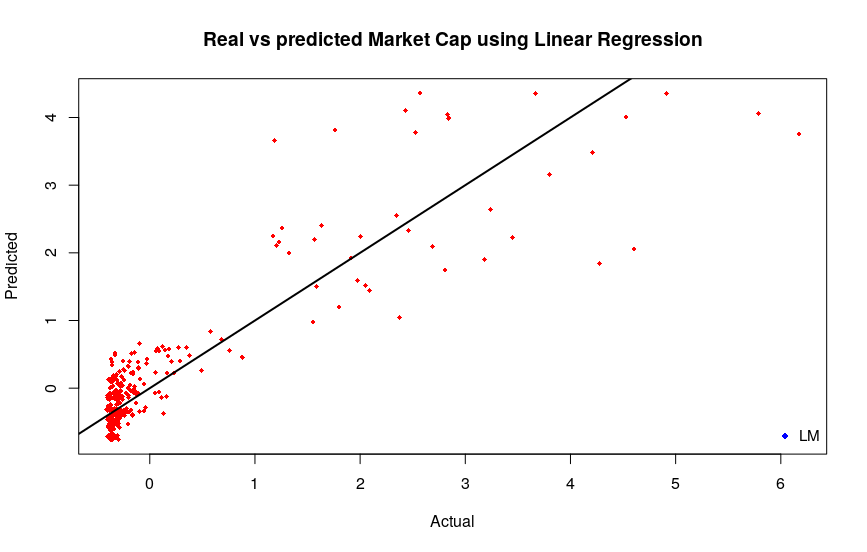
\includegraphics[width=\linewidth]{MarketCapLR}
	\caption{Bitcoin Market Cap Prediction based on Open Price}
	\label{fig1:MarketCapLR}
\end{figure}
\newpage

\subsection {Visualizing Using Tableau}
\subsubsection{Inferences for Various Visualizations Performed on Different Attributes}
We explored the variation of various attributes of cryptocurrencies (Bitcoin and Ethereum) and the impact on their use worldwide:
\begin{itemize}

\item The hash rate of a cryptocurrency is a measure of how many \textbf{proof of work} calculations are being performed by all the miners participating in the network. It is measured in terms of number hashes per second, but because such a large number of these calculations are performed, it is more usual to see values in larger units such as Gigahashes per second (GHS) or Terrahashes per second (THS).
That means, if a cryptocurrency network has a low hash rate, then the cost for an attacker wanting to purchase enough hashing power to attack the network would be relatively low. As the hash rate goes up, so does the cost of attacking the network. 
Knowing this correlation would help a network of miners avoid any fraudulent transaction by a malicious miner.

\begin{figure}[h]
    \centering
    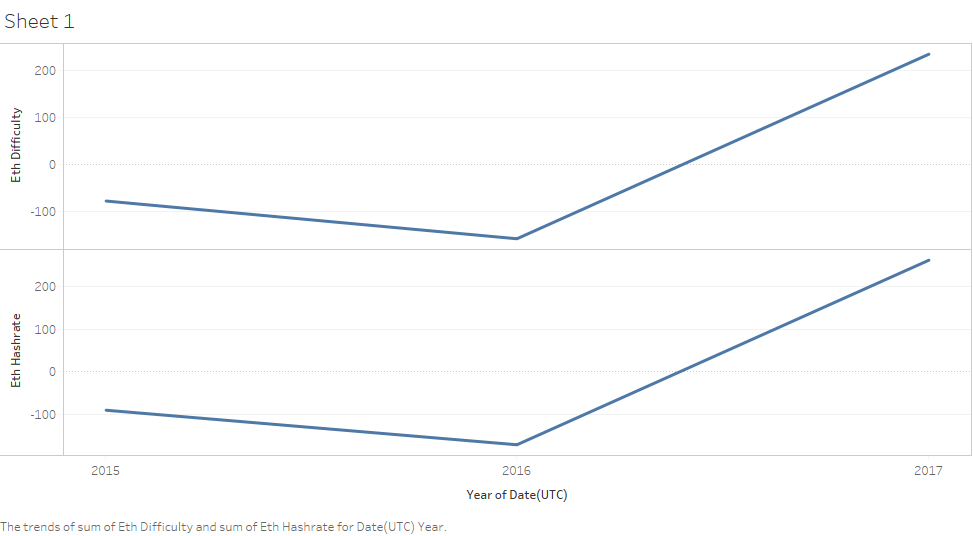
\includegraphics[width=10cm]{eth_hashrate_difficulty.png}
    \caption{Variation of Ethereum's Hashrate and Difficulty attributes with time}
    \label{fig:my_label}
\end{figure}

\newpage
\begin{figure}[h]
    \centering
    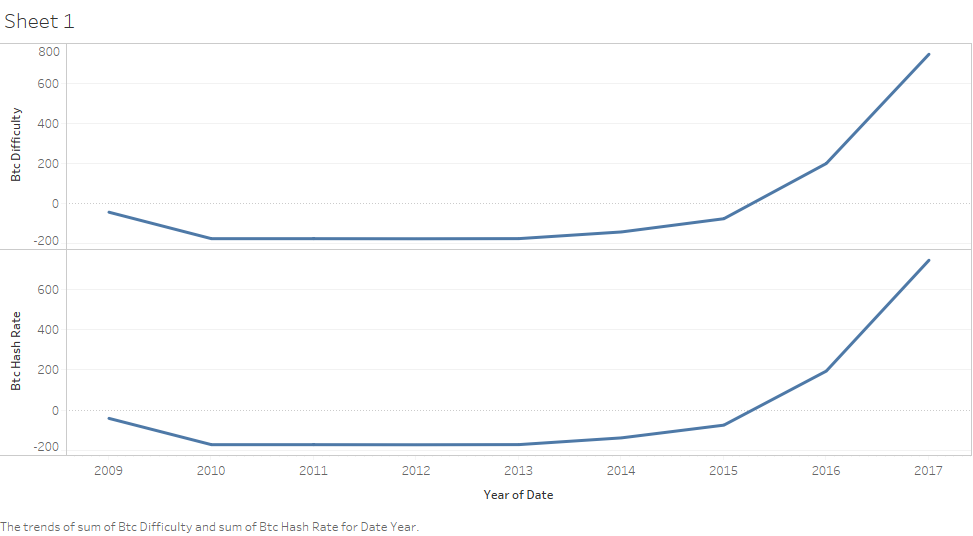
\includegraphics[width=10cm]{btc_difficulty_hashrate.png}
    \caption{Variations of Bitcoin's Difficulty and Hashrate attributes with time}
    \label{fig:my_label}
\end{figure}

\item When the number of transaction increases, more blocks are produced. Since there is a cap of average 1 block per 10 minutes, the difficulty of the network increases. With the difficulty increase, the hashrate has to increase to keep generating blocks on time. Hence, it can be inferred that with increase in hashrate, the difficulty increases as well because with number of transactions, the hashrate has to increase to keep processing them. With the hashrate increased blocks are generated faster and thus difficulty is increased.
This knowledge helps maintain a balance between number of transactions and difficulty, so that neither is the number of transactions too high, leading to high difficulty, neither is it too low, leading to an inverse causation on market price.
\begin{figure}[h]
    \centering
    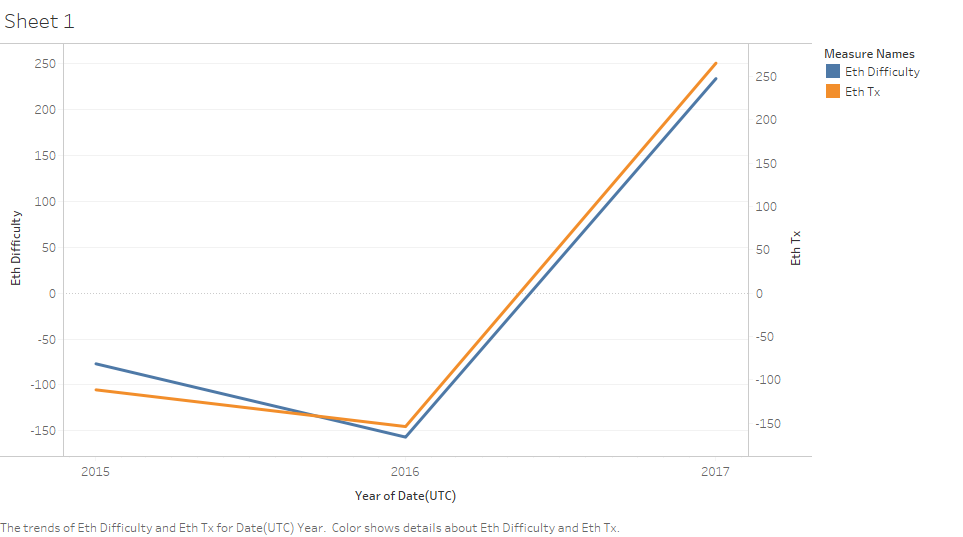
\includegraphics[width=10cm]{eth_transactions_difficulty.png}
    \caption{Variation of Number of Transactions and Difficulty attributes of Ethereum with time}
    \label{fig:my_label}
\end{figure}

\newpage
\begin{figure}[h]
    \centering
    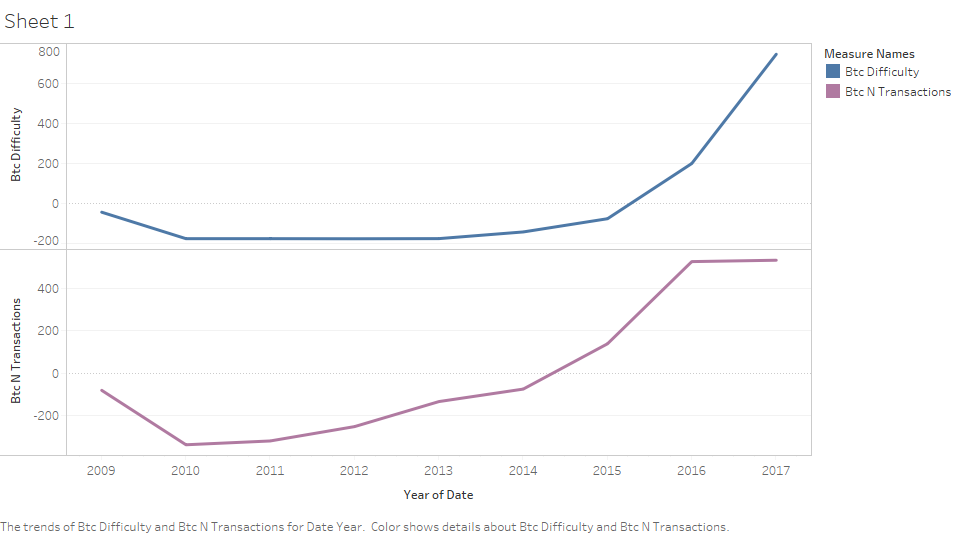
\includegraphics[width=10cm]{btc_transactions_difficulty.png}
    \caption{Variation of Bitcoin's Number of Transactions and Difficulty attributes with time}
    \label{fig:my_label}
\end{figure}

\item There is a long-run feedback cycle between difficulty and price. If the price goes up, that makes mining more lucrative, and people buy new hardware to capitalize on that. As a result, the hashing power increases, however, there’s actually a temporary increase in the daily bitcoin production, thereby causing an increase in the supply. This occurs because difficulty only adjusts every 2016 blocks, so as mining power increases it takes difficulty to catch up in some time and in the meantime, blocks are produced more frequently than once per 10 minutes target rate. We plotted the correlation trends of the features in the Ethereum's dataset with it's market price and measured the correlation coefficients for each of them. 
\newpage
As expected, it turns out that the top 5 features affecting the ethereum's price are:
\begin{enumerate}
\item \textbf{Eth Hashrate:} Hashrate in Giga hashes per second.
\item \textbf{Eth Difficulty:} Difficulty level 
\item \textbf{Eth address:} Cumulative address growth
\item \textbf{Eth Blocksize:} Average block size in bytes
\item \textbf{Eth Marketcap:} Market Capitalization in USD
\end{enumerate}
Above realisation helps in more accurate predictions about the cryptocurrencies' price, now that we know the major price drivers.
\begin{figure}[h]
    \centering
    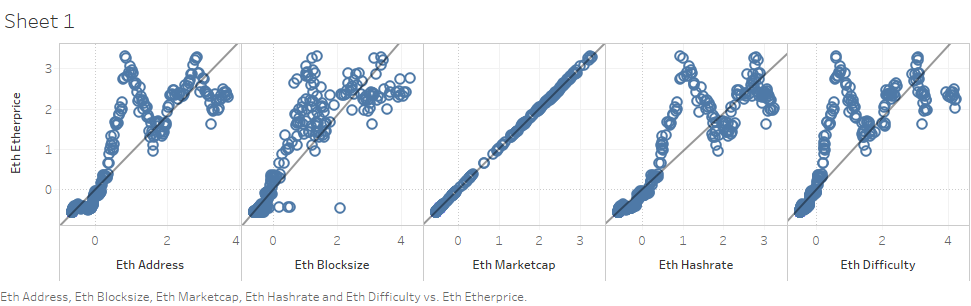
\includegraphics[width=11cm]{correlation_coefficient.png}
    \caption{Correlation of Ethereum's attributes with the Ethereum Market Price}
    \label{fig:my_label}
\end{figure}

\item For analyzing the correlations between multiple cryptocurrencies (Bitcoin and Ethereum), we performed inner-join on the Data Sets of the respective cryptocurrencies on Date attribute. This was followed by plotting the market price of these cryptocurrencies with the time dimension. As revealed by the tableau visualizations, the market price of the two are highly correlated with each other, as both simultaneously takes a dip and then increase with time. This process could be followed for the other cryptocurrencies to understand their mutual correlation with each other and the market.
It can be seen that investors can use their knowledge about one cryptocurrency to infer behaviour of the other.

\begin{figure}[h]
    \centering
    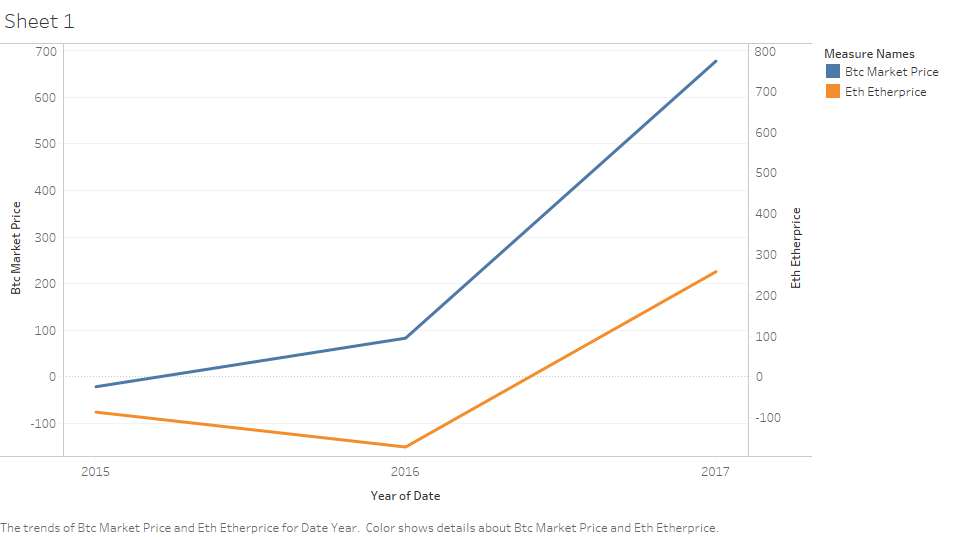
\includegraphics[width=10cm]{btc_eth_price_date.png}
    \caption{Variation of Bitcoin and Ethereum's Market Price with Date attribute}
    \label{fig:my_label}
\end{figure}

\newpage
Similarly, plotting the Volume attribute of former cryptocurrencies with the time dimensions shows similar results as above, confirming our inferences.
\begin{figure}[h]
    \centering
    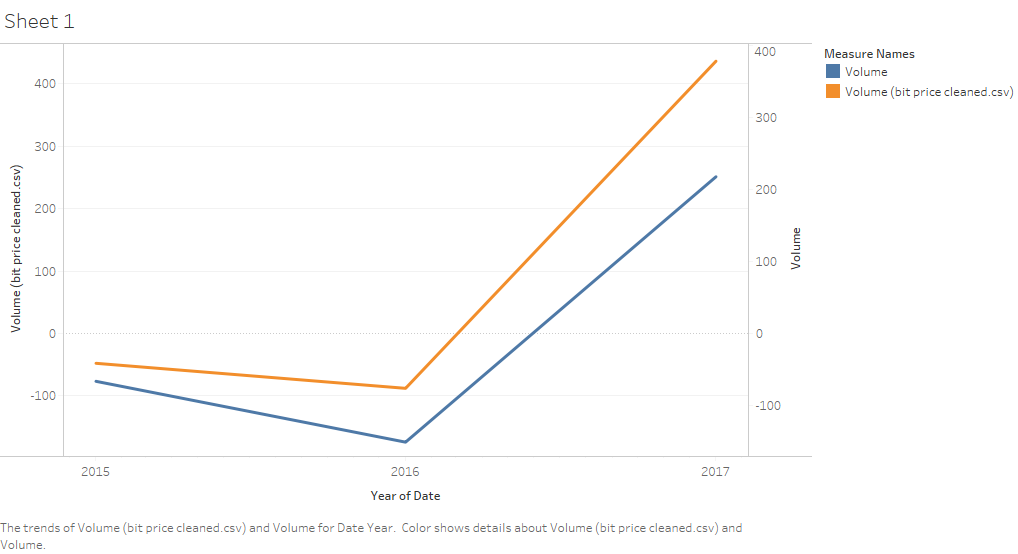
\includegraphics[width=10cm]{bit_eth_volume.png}
    \caption{Variation of Bitcoin and Ethereum's Volume with Date attribute}
    \label{fig:my_label}
\end{figure}

\item From the historical behaviour of the cryptocurrencies, we know that hash rate increases with the number of transactions, and in turn Difficulty also increases.  As seen from the plot below between the transaction fees paid to miners (validating the transactions) and the median time for a transaction to be accepted into a mined block, it can be inferred that with increase in the transaction fees, the median time also seems to be increasing, however not with similar rate. Thus, the visualizations below confirms our hypothesis that with increase in number of transactions, transaction fees increases and hence average confirmation time also rises.
This would help miners verify if the transactions fees paid to them is fair according to the time spent on a block.

\begin{figure}[h]
    \centering
    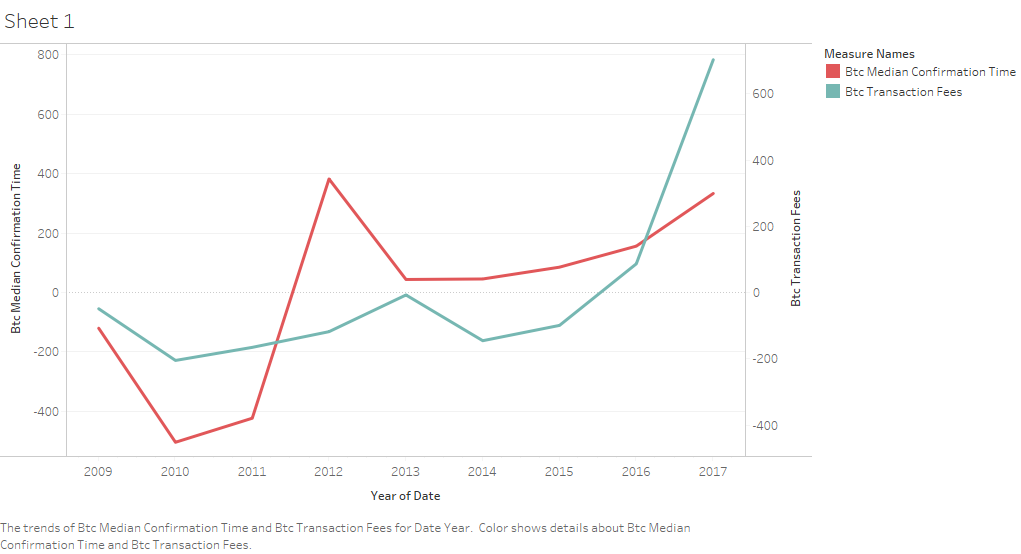
\includegraphics[width=10cm]{btc_transaction_fees_avg_time.png}
    \caption{Variation of Bitcoin's Transaction Fees attribute with Median Confirmation Time attribute}
    \label{fig:my_label}
\end{figure}

\end{itemize}


\section{References}

\begin{enumerate}

\item Feature Selection and Classification Techniques for Multivariate Time Series
Basabi Chakraborty ;Faculty of Software and Information Science, Iwate Prefectural University - 152-52 Sugo, Takizawa-mura, Iwate, 020-0193, Japan E-mail: basabi@soft.iwate-pu.ac.jp.\newline

\item http://www.rdatamining.com/examples/time-series-clustering-classification.\newline

\item The Application of Machine Learning Techniques to Time-Series Data - Author Scott Mitchell; Master of Computing and Mathematical Sciences at the University of Waikato. \newline

\item Article by Sunil Ray at Analytics Vidhya Website

\item Predicting the direction of stock market prices using random forest. Luckyson Khaidem Snehanshu Saha Sudeepa Roy Dey. khaidem90@gmail.com snehanshusaha@pes.edu sudeepar@pes.edu

\item Forecasting of Indian Stock Market Index Using Artificial Neural Network Manna Majumder1 , MD Anwar Hussian2

\item Stock Price Prediction Using Regression Analysis Dr. P. K. Sahoo, Mr. Krishna charlapally

\item Random Forests by the founders ; Leo Breiman and Adele Cutler

\item rstudio-pubs website describing about the Random Forest.

\item Article published at the Tutor website for R tutorial.


\item Article published at the Institute for Digital Research and Education website.

\item Article from the pdf https://www.epa.gov/sites/production/files/2016-07/documents/regression.pdf

\item Article published at http://erickokellostatcentre.blogspot.in/2016/06/simple-linear-regression-pros-and-cons.html

\item Paper on Automated Bitcoin Trading via Machine Learning Algorithms 

\item www.cryptorial.io

\end{enumerate}

\end{document}

